\documentclass{article}

\usepackage{tikz} 
\usetikzlibrary{automata, positioning, arrows} 

\usepackage{amsthm}
\usepackage{amsfonts}
\usepackage{amsmath}
\usepackage{amssymb}
\usepackage{fullpage}
\usepackage{color}
\usepackage{parskip}
\usepackage{hyperref}
  \hypersetup{
    colorlinks = true,
    urlcolor = blue,       % color of external links using \href
    linkcolor= blue,       % color of internal links 
    citecolor= blue,       % color of links to bibliography
    filecolor= blue,        % color of file links
    }
    
\usepackage{listings}

\graphicspath{ {./images/} }

\definecolor{dkgreen}{rgb}{0,0.6,0}
\definecolor{gray}{rgb}{0.5,0.5,0.5}
\definecolor{mauve}{rgb}{0.58,0,0.82}

\lstset{frame=tb,
  language=haskell,
  aboveskip=3mm,
  belowskip=3mm,
  showstringspaces=false,
  columns=flexible,
  basicstyle={\small\ttfamily},
  numbers=none,
  numberstyle=\tiny\color{gray},
  keywordstyle=\color{blue},
  commentstyle=\color{dkgreen},
  stringstyle=\color{mauve},
  breaklines=true,
  breakatwhitespace=true,
  tabsize=3
}

\newtheoremstyle{theorem}
  {\topsep}   % ABOVESPACE
  {\topsep}   % BELOWSPACE
  {\itshape\/}  % BODYFONT
  {0pt}       % INDENT (empty value is the same as 0pt)
  {\bfseries} % HEADFONT
  {.}         % HEADPUNCT
  {5pt plus 1pt minus 1pt} % HEADSPACE
  {}          % CUSTOM-HEAD-SPEC
\theoremstyle{theorem} 
   \newtheorem{theorem}{Theorem}[section]
   \newtheorem{corollary}[theorem]{Corollary}
   \newtheorem{lemma}[theorem]{Lemma}
   \newtheorem{proposition}[theorem]{Proposition}
\theoremstyle{definition}
   \newtheorem{definition}[theorem]{Definition}
   \newtheorem{example}[theorem]{Example}
\theoremstyle{remark}    
  \newtheorem{remark}[theorem]{Remark}

\title{CPSC-354 Report}
\author{Emma Garofalo  \\ Chapman University}

\date{\today} 

\begin{document}

\maketitle

\begin{abstract}
This document outlines what has been learned week by week through this class. For now, it only contains the information learned for week one.
\end{abstract}

\setcounter{tocdepth}{3}
\tableofcontents

\section{Introduction}\label{intro}
Welcome to my class report! As the class progresses, I will add my learning
from each week. For now, it only has week one. 
\section{Week by Week}\label{homework}

\subsection{Week 1}
\subsubsection*{Notes}
This week we discussed the foundation of what the class is about.
The main idea was that this class is largely about the intersection
of math and programming, beginning with revisiting the principles we learned
in discrete mathematics. We also learned about LaTeX, which we will be using throughout 
the semester to edit documents like this one. The general idea of the week was setting all of us 
students up for what to expect throughout the semester.

We also covered the topics of Formal Systems, which are explained in more detail in the below
section. And how to determine the relations between a Lean proof and a Math proof.
\subsubsection*{Homework}

The reading that we had to cover for homework discussed the MUI problem, which helps us
break down what a formal system is, and how these attributes can be seen in mathematics like 
discrete math. A formal system carries the requirement of formality, which states that you
must not do anything outside of the set rules. Theorems, axioms, rules of production, and the
decision procedure are all key parts of a formal system.

We also had to complete the tutorial world of the natural number game. 
Here are the solutions for levels 5-8.

\subsubsection*{Level 5}
Goal: a+(b+0)+(c+0)=a+b+c

Solution:
\begin{lstlisting}
rw[add_zero]
rfl
\end{lstlisting}
\subsubsection*{Level 6}
Goal: a+(b+0)+(c+0)=a+b+c

Solution:
\begin{lstlisting}
rw[add_zero c]
rw[add_zero]
rfl
\end{lstlisting}
\subsubsection*{Level 7}
Goal: succ n = n + 1

Solution:
\begin{lstlisting}
rw[one_eq_succ_zero]
rw[add_succ]
rw[add_zero]
rfl
\end{lstlisting}
\subsubsection*{How is this lean proof related to mathematics proofs?:}
The definition of Natural Numbers. 
1. "There is a special natural number, called zero, denoted by 0."
2. "For any natural number n, there is a unique next natural number, called
the successor of n."

\begin{align}
succ n &= n + 1         &   \\
succ n &= n + succ(0)   &    &\text{definition of natural numbers} \\
succ n &= succ(n + 0)   &    &\text{prop. of + for successors} \\
succ n &= succ n        &    &\text{additive identity property} \\
\end{align}
\subsubsection*{Level 8}
Goal: 2 + 2 = 4

Solution:
\begin{lstlisting}
nth_rewrite 2[two_eq_succ_one]
rw[one_eq_succ_zero]
rw[four_eq_succ_three]
rw[three_eq_succ_two]
nth_rewrite 2[two_eq_succ_one]
rw[one_eq_succ_zero]
rw[two_eq_succ_one]
rw[one_eq_succ_zero]
rw[add_succ]
rw[add_succ]
rw[add_zero]
rfl
\end{lstlisting}

I learned a lot from this homework. It basically acted as a refresher for discrete mathematics, and 
how what seems like such a simple solution is much more complicated than you think it is. It also shows 
the various ways that you can derive the same solutions.


\subsubsection*{Comments and Questions}

This week provided me with a good refresher of the discrete mathematics class that I took a while ago. It brought to my attention how much
there is a crossover between math and code, and I am so excited to explore that in this class.

My question for the week relates to the foundation of mathematics, and where it has all evolved from there. We refreshed on discrete math,
which shows us why even the simplest mathematic proofs are valid. And it makes me wonder how mathematics has evolved so much since then. We have
such calculated math that has all built off of these proofs. Seeing how much math has evolved since then, does that mean that math will continue to
evolve in complexity forever? As we create new technologies and understand our world better, will more complicated relationships continue to be found?

\subsection{Week 2: Recursion}
\subsubsection*{Notes}
The main topic of this week was recursion, and how it can be visualized with the "Tower of Hanoi" exercise.
We learned that the definition of recursion is nesting, and variations on nesting. Recursive definitions are
defined in simpler terms of itself, but they never lead to infinite regress or paradox. The "Tower of Hanoi" showed
us this well by demonstrating that once you find a base case (a simpler way to break the problem down), then you can
use that and the successor of that to solve recursively. We considered the problem from the bottom disk up, and observed
how both a stack machine and a rewriting machine can find the efficient recursive solutions.

\subsubsection*{Homework}
The reading that we had for homework was about the "Little Harmonic Labyrinth". This story was a complex example of how
recursion is nesting, and variations on nesting. Another real life example that this reading provided was postponing the 
completion of a task in favor of completing a simpler task, which I think is something that humans naturally do all the time.

We also completed the addition world of the Natural Number Game, and some solutions are outlined below.
\subsubsection*{Level 1}
Goal: 0 + n = n

Solution:
\begin{lstlisting}
induction n with d hd
rw[add_zero]
rfl

rw[add_succ]
rw[hd]
rfl
\end{lstlisting}
\subsubsection*{Level 2}
Goal: succ a + b = succ (a + b)

Solution:
\begin{lstlisting}
induction b with n hn
rw[add_zero]
rw[add_zero]
rfl

rw[add_succ]
rw[hn]
rw[add_succ]
rfl
\end{lstlisting}
\subsubsection*{Level 3}
Goal: a + b = b + a

Solution:
\begin{lstlisting}
induction b with d hd
rw[add_zero]
rw[zero_add]
rfl

rw[add_succ]
rw[hd]
rw[succ_add]
rfl
\end{lstlisting}
\subsubsection*{Level 4}
Goal: a + b + c = a + (b + c)

Solution:
\begin{lstlisting}
induction c with d hd
rw[add_zero]
rw[add_zero]
rfl

rw[add_succ]
rw[hd]
rw[add_succ]
rw[add_succ]
rfl
\end{lstlisting}
\subsubsection*{How is this lean proof related to mathematics proofs?:}
\begin{align}
  a + b + c = a + (b+c)   &      &\text{proof by induction on c} \\
  a + b + 0 = a + (b+0)   &      &\text{base case} \\
  a + b = a + b        &      &\text{additive identity} \\
  succ(a + b + d) = a + (b+succd)&    &\text{inductive step} \\
  succ(a + (b + d)) = a + (b+succd)&      &\text{substitution with inductive hypothesis} \\
  succ(a + (b + d)) = succ(a + (b+d))&      &\text{prop. of + for successors} \\
\end{align}


Then the identity property for addition is performed, showing that a + 0 = a.
Once the base case is proven, the successor must be proven as well.
The property of addition for successors simplifies the goal so that the inductive hypothesis can 
be substituted. With another simplification from the addition of successors, both sides of the equation
are shown to be equivalent.
\subsubsection*{Level 5}
Goal: a + b + c = a + c + b

Solution:
\begin{lstlisting}
induction c with d hd
rw[add_zero]
rw[add_zero]
rfl

rw[add_succ]
rw[add_succ]
rw[hd]
rw[succ_add]
rfl
\end{lstlisting}
This homework was all about recursion. It refreshed my knowledge on how to apply induction
to reach the goal.

\subsubsection*{Comments and Questions}
The "Tower of Hanoi" problem reminded me the give and take when it comes to finding 
recursive solutions. Oftentimes, a recursive solution is a more efficient one, but the time
it takes to think up this solution and the possible complexity of it needs to be taken into consideration.

My question of the week relates to this. Is there a key way to always identify that the most efficient solution to
a particular problem is recursion? I feel like when a problem becomes more complicated, I struggle to identify if 
it can be solved recursively, and because of this, I try multiple other solutions before and waste a lot of time
coming to a recursive solution.

\subsection{Week 3: Programming with LLMs}
\subsubsection*{Notes}
LLMs for literature reviews 

Start discussing creating a calculator in python
\subsubsection*{Homework}

The homework for this week had us focus on how to use LLMs effectively. We had to have
a conversation with an LLM of our choice, and use it to create a literature review
on a topic of our choosing related to programming languages. 

\href{https://github.com/egarof00/CPSC354-HW3}{My literature review}:
I covered the topic of programming languages in video game design. The README is linked in the title above. 
I also wrote a more detailed summary in my discord posting \href{https://discord.com/channels/1277862531226013750/1278164700076707892/1285026014057070632}{here},
under the name MagicTurtle. These documents follow the general trajectory that programming languages have taken over time, and how
they have been used and improved. It also covers the general strengths of the common programming languages used today, and why
they are better for particular types of games than others.

\subsection*{Other Literature Reviews That I Found Interesting:}
\href{https://github.com/keira-ryan/question/blob/main/README.md}{Programming Languages and Art}

Author: Keira Ryan 
As someone who is not as familiar with art, this literature review was very interesting to me.
I think that it took a very good stance on the hot topic of AI art and whether or not
it is "real". It explains that AI can be used as a tool in the art world, and a way to 
experiment with new processes. 

\href{https://github.com/cjoo03/HW3/blob/main/README.md}{Exploring Garbage Collection Across Programming Languages}

Author: Chris Joo
I found this interesting because it is an aspect of programming that is often overlooked.
It is an extremely important part of programming, but when it is taken care of, I often
do not think twice about how it is accomplished. 


\subsubsection*{Comments and Questions}

This week provided me with a good refresher of the discrete mathematics class that I took a while ago. It brought to my attention how much
there is a crossover between math and code, and I am so excited to explore that in this class.

My question for the week relates to the foundation of mathematics, and where it has all evolved from there. We refreshed on discrete math,
which shows us why even the simplest mathematic proofs are valid. And it makes me wonder how mathematics has evolved so much since then. We have
such calculated math that has all built off of these proofs. Seeing how much math has evolved since then, does that mean that math will continue to
evolve in complexity forever? As we create new technologies and understand our world better, will more complicated relationships continue to be found?


\subsection{Week 4: Parsing and Context-Free Grammars}
\subsubsection*{Notes}
Concrete syntax vs. abstract syntax

Parsing

Context-Free Grammar

Caculator with parser generator
\subsubsection*{Homework}

We did various different assignments for homework this week. The first is shown below.
Using this context-free grammar
\begin{lstlisting}
  Exp -> Exp '+' Exp1 
  Exp1 -> Exp1 '*' Exp2              
  Exp2 -> Integer            
  Exp2 -> '(' Exp ')'  
  Exp -> Exp1             
  Exp1 -> Exp2 
\end{lstlisting}
write out derivation/parse trees for each string:
\begin{enumerate}
  \item 2+1
  \item 1+2*3
  \item 1+(2*3)
  \item (1+2)*3
  \item 1+2*3+4*5+6
\end{enumerate}
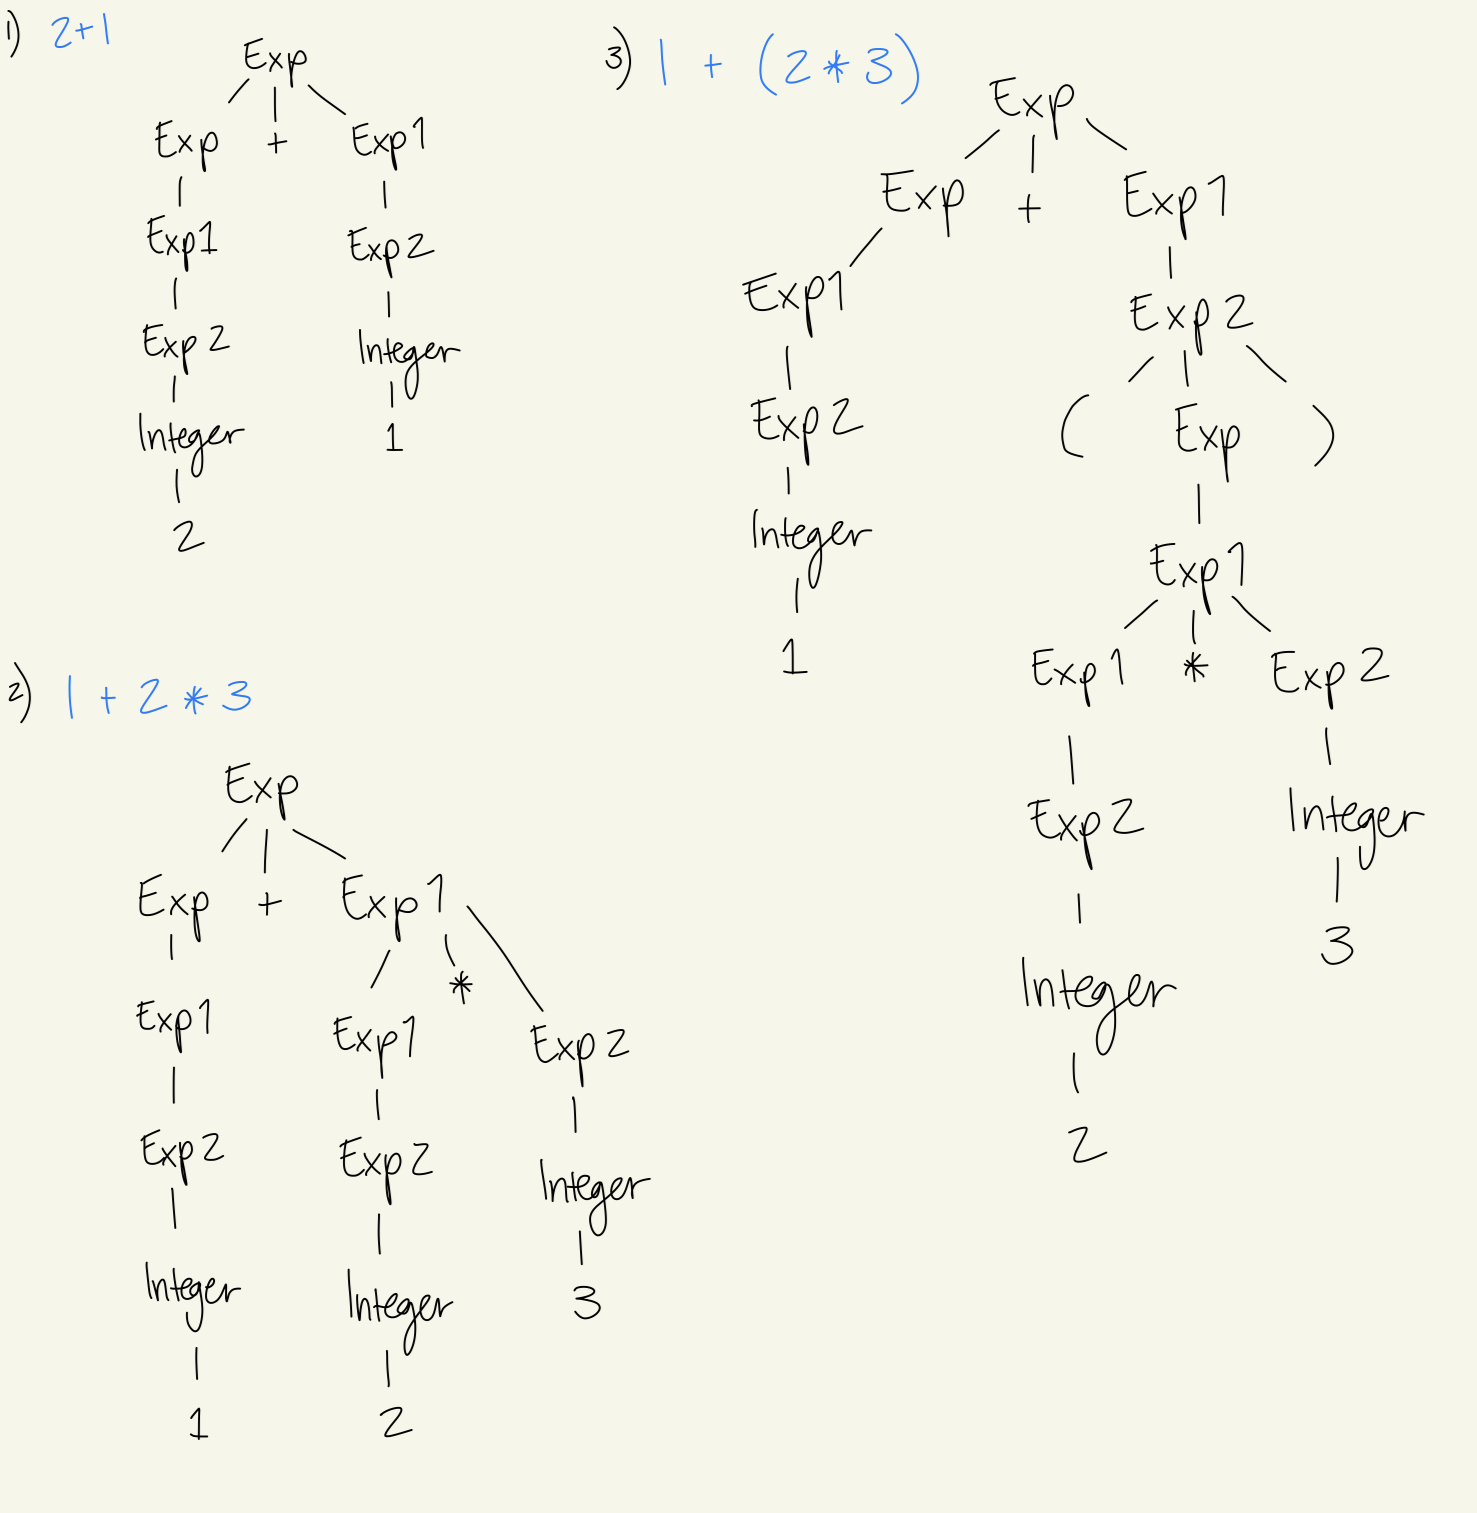
\includegraphics[scale=0.15]{IMG_1712}
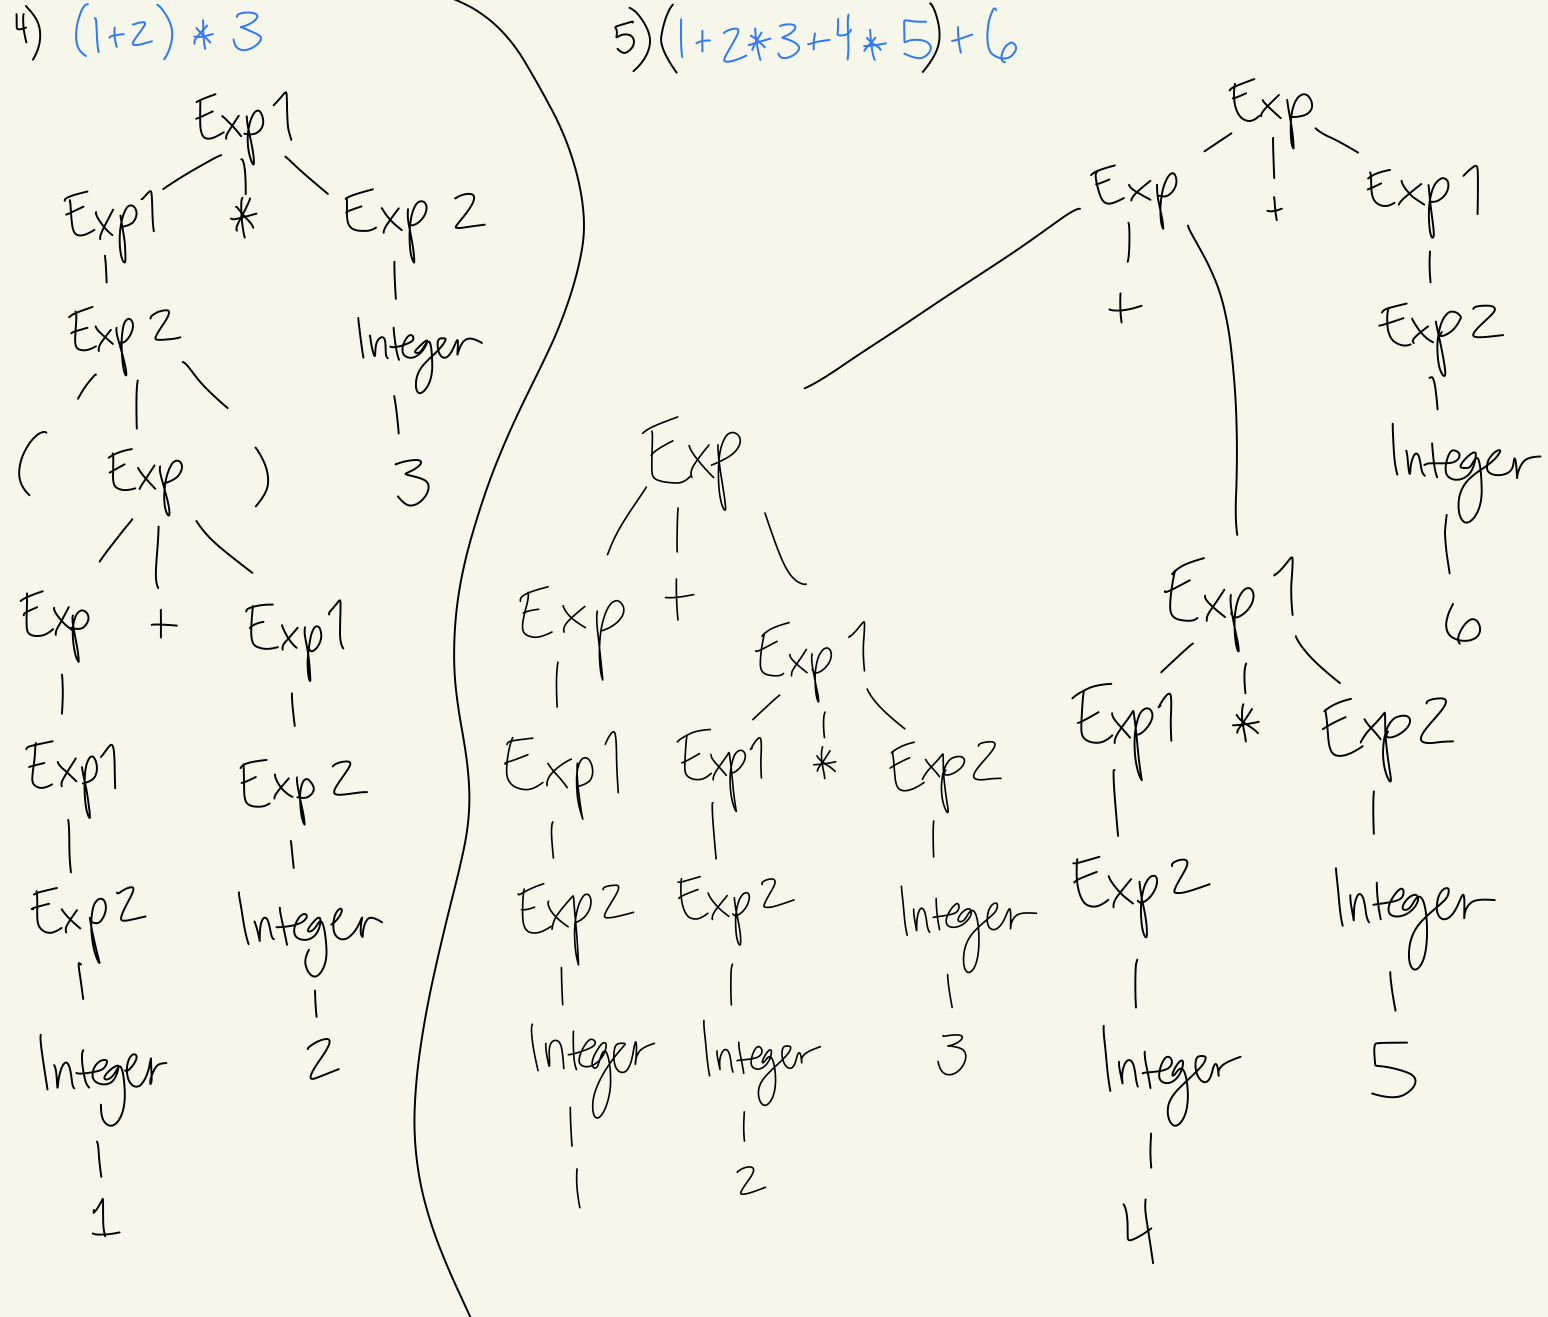
\includegraphics[scale=0.15]{IMG_1713}

We also worked on creating a calculator in python that completes basic math 
operations (parentheses, exponents, multiplication, subtraction, and addition). 
We did this our own way, but we discussed that a great way to complete this project would be 
by creating a parser generator in a software like Lark. 

The reading this week went into detail on the topic of parsing and context free grammars. These context 
free grammars are basically sets of rules that are created to define a language. They must be grammatically 
defined by four components: a finite set of symbols, finite set of variables, a start symbol, and a finite set of
productions. From these, you can perform either recursive inferences or derivations. 
\subsubsection*{Comments and Questions}
This week focused a lot on breaking down what defines a context free grammar and all of the very complicated
details that make up a CFG. The topic puts a lot of focus on what is allowed in a context free grammar, so
I wanted to instead focus on the exclusions from these languages and how they are identified. When a CFG is 
used for a programming language syntax, how is it able to give meaningful error messages? Is it able to 
identify what part of the language that a string would not be valid for and then give an error message in
relation to that? I am just unsure overall of how meaningful error messages are given when a CFG is used
because it is something I have never really thought about until now. 

\subsection{Week 5: Propositions as Types, Dependent Types}
\subsubsection*{Notes}
This week we discussed a LARL (look-ahead, left to right, rightmost derivation parser). This kind of parser
moves all the way to the right when performing a derivation in  order to perform the rightmost derivation first.
In its derivation, it can only perform two actions: shift or reduce. Sometimes this creates shift-reduce conflicts.

\subsubsection*{Homework}
For homework we worked on programming assigment 2, which started with the base of a python calculator script
and lark parsing grammar. Our goal was to add operations to this base while being sure that the order of 
operations was respected, even for long mathematical expressions. For each added expression, we went through the 
steps of adding the operation to the grammar (in the correct order), adding that operation to the python transformer
function, then adding it to the evaluator. Each new operation needed to be tested both on its own and with other
operations in order to ensure that they functioned correctly and respected the order of operations.

We also completed the tutorial world of the Lean Logic Game. This showed how to solve problems in a language
that operates only with variables and functions. No data types or memory exist. The solutions to the tutorial 
world are shown below:
\subsubsection*{Level 1}
\begin{lstlisting}
(P : Prop)(todo_list : P) : P := by
\end{lstlisting}
Solution:
\begin{lstlisting}
  exact todo_list
\end{lstlisting}
\subsubsection*{Level 2}
\begin{lstlisting}
(P S : Prop)(p: P)(s : S) : P /\ S := by
\end{lstlisting}
Solution:
\begin{lstlisting}
  exact <p,s>
\end{lstlisting}
\subsubsection*{Level 3}
\begin{lstlisting}
(A I O U : Prop)(a : A)(i : I)(o : O)(u : U) : (A /\ I) /\ O /\ U := by
\end{lstlisting}
Solution:
\begin{lstlisting}
  exact <<a,i> , o, u>
\end{lstlisting}
\subsubsection*{Level 4}
\begin{lstlisting}
(P S : Prop)(vm: P /\ S) : P := by
\end{lstlisting}
Solution:
\begin{lstlisting}
  exact vm.left : p
\end{lstlisting}
\subsubsection*{Level 5}
\begin{lstlisting}
(P Q : Prop)(h: P /\ Q) : Q := by
\end{lstlisting}
Solution:
\begin{lstlisting}
  exact h.right
\end{lstlisting}
\subsubsection*{Level 6}
\begin{lstlisting}
(A I O U : Prop)(h1 : A /\ I)(h2 : O /\ U) : A /\ U := by
\end{lstlisting}
Solution:
\begin{lstlisting}
  exact <h1.left, h2.right>
\end{lstlisting}
\subsubsection*{Level 7}
\begin{lstlisting}
(C L : Prop)(h: (L /\ (((L /\ C) /\ L) /\ L /\ L /\ L)) /\ (L /\ L) /\ L) : C := by
\end{lstlisting}
Solution:
\begin{lstlisting}
  have h1 := h.left
  have h2 := h.right
  have h4 := h1.right
  have h5 := h4.left
  have h6 := h5.left
  exact h6.right
\end{lstlisting}
\subsubsection*{Level 8}
\begin{lstlisting}
(A C I O P S U : Prop)(h: ((P /\ S) /\ A) /\ -I /\ (C /\ -O) /\ -U) : A /\ C /\ P /\ S := by
\end{lstlisting}
Solution:
\begin{lstlisting}
  have h1 := h.left
  have h2 := h1.left
  have h3 := h1.right
  have h4 := h.right
  have h5 := h4.right
  have h6 := h5.left
  have h7 := h6.left
  exact <h3, h7, h2>
\end{lstlisting}
\subsubsection*{How is this lean proof related to mathematics proofs?:}
\begin{align}
  have h1 := h.left   &      &\text{isolate  (P AND S) AND A} \\
  have h2 := h1.left   &      &\text{isolate P AND S} \\
  have h3 := h1.right        &      &\text{isolate A} \\
  have h4 := h.right&    &\text{isolate I AND (C AND ¬O) AND ¬U} \\
  have h5 := h4.right&      &\text{isolate (C AND ¬O) AND ¬U} \\
  have h6 := h5.left&      &\text{isolate C AND ¬O} \\
  have h7 := h6.left&      &\text{isloate C} \\
  exact <h3, h7, h2>&      &\text{and intro} \\
\end{align}

The goal of this problem is to break down the hypothesis into smaller chunks that are
already known in order to prove that it is true. Once we get to the digestable values
of P AND S, C, and A. We are then able to show that if these are each true individually,
then they can be combined to also all be true.

\subsubsection*{Comments and Questions}
This week we went into parsing trees a bit more in our lecture, and one of the 
things that we talked about were LARLs, or look ahead/rightmost derivation trees.
It is one of the kinds of predictive parsing, but it made me wonder what situations
this type of parsing is actually used, and how it could possibly be flexible in any way. 
Does relying on rightmost derivation limit it's effeciency to very particular problems?
Or is their a way to make it more flexible so that it can handle left-recursive 
grammars just as well?

\subsection{\ldots}

\subsection{Week 6: Higher Order Functions}
\subsubsection*{Notes}
The topics of this week mostly included currying and lambda calculus. In class, we discussed that currying is like
creating a chain of functions in order to solve a particular problem. This is done because in the scenarios 
that it is used, each function only takes in one argument. 

We also focused a lot of lambda calculus, which as we previously discussed, is made up of only vaiables 
and functions. In order to dive deeper into the topic, we broke it down into syntax and semantics. 
The syntax of lambda caclulus is what I have below. The bottom two being abstraction and application, respectively.
\begin{lstlisting}
  exp -> var
  exp -> 'lambda' var '.' exp
  exp -> exp exp 
\end{lstlisting}

The operational semantics of lambda calculus, otherwise known as how programs will run, was broken down 
when observing the proof of an identity function. We stressed that each function is only able to take
one input, and observing parenthesis properly while using substitution with capture avoiding is necessary
in lambda calculus.
\subsubsection*{Homework}
This week's homework was the "Party Snacks" level of the lean logic world, focusing on lambda calculus. 
We pushed ourselves to solve each problem in a single line. The solutions to problems 1-9 are shown below:
('lambda' and 'maps to' symbols are represented in text because of latex restrictions)
\subsubsection*{Level 1}
\begin{lstlisting}
(P C: Prop)(p: P)(bakery_service : P -> C) : C := by
\end{lstlisting}
Solution:
\begin{lstlisting}
  exact bakery_service p
\end{lstlisting}
\subsubsection*{Level 2}
\begin{lstlisting}
  (C: Prop) : C -> C
\end{lstlisting}
Solution:
\begin{lstlisting}
  exact 'lambda' c 'maps to' c
\end{lstlisting}
\subsubsection*{Level 3}
\begin{lstlisting}
(I S: Prop) : I /\ S -> S /\ I
\end{lstlisting}
Solution:
\begin{lstlisting}
  exact 'lambda' <I, S> 'maps to' <S, I>
\end{lstlisting}
\subsubsection*{Level 4}
\begin{lstlisting}
(C A S: Prop) (h1 : C -> A) (h2 : A -> S) : C -> S
\end{lstlisting}
Solution:
\begin{lstlisting}
  exact 'lambda' c 'maps to' h2 (h1 c)
\end{lstlisting}
\subsubsection*{Level 5}
\begin{lstlisting}
(P Q R S T U: Prop) (p : P) (h1 : P -> Q) (h2 : Q -> R) (h3 : Q -> T) (h4 : S -> T) (h5 : T -> U) : U
\end{lstlisting}
Solution:
\begin{lstlisting}
  exact h5 (h3 (h1 p))
\end{lstlisting}
\subsubsection*{Level 6}
\begin{lstlisting}
(C D S: Prop) (h : C /\ D -> S) : C -> D -> S
\end{lstlisting}
Solution:
\begin{lstlisting}
  exact 'lambda' c d 'maps to' h <c, d>
\end{lstlisting}
\subsubsection*{Level 7}
\begin{lstlisting}
(C D S: Prop) (h : C -> D -> S) : C /\ D -> S
\end{lstlisting}
Solution:
\begin{lstlisting}
  exact 'lambda' <c, d> 'maps to'  h c d
\end{lstlisting}
\subsubsection*{Level 8}
\begin{lstlisting}
(C D S : Prop) (h : (S -> C) /\ (S -> D)) : S -> C /\ D
\end{lstlisting}
Solution:
\begin{lstlisting}
  exact 'lambda' s 'maps to'  <h.left s, h.right s> 
\end{lstlisting}
\subsubsection*{Level 9}
\begin{lstlisting}
(R S : Prop) : R -> (S -> R) /\ (-S -> R)
\end{lstlisting}
Solution:
\begin{lstlisting}
  exact 'lambda' r 'maps to' <'lambda' s 'maps to' r, 'lambda' ns 'maps to' r>
\end{lstlisting}


\subsubsection*{Comments and Questions}
One of the topics generally mentioned this week was the Curry-Howard correspondence.
It demonstrates a connection between formal systems of logic and programming languages,
stating that a propositions correspond to types, proofs correspond to programs, and proof reductions
correspond to program evaluation. It is able to show the direct connections between mathematics 
and programming. My question for the week is how can this understanding improve our approach to
programming?

\subsection{Week 7}
\subsubsection*{Notes}
This week we covered why lambda calculus is turing complete. We wanted to show how to represent
numbers, operations, conditionals, memory, and loops. We also observed recursion in lambda calculus.

\subsubsection*{Homework}
For homework, we had to practice capture avoiding substitution. We were tasked with this problem:

1. Reduce the following lambda term:
\begin{lstlisting}
  ((\m. \n. m n) (\f. \x. f (f x))) (\f. \x. f (f (f x))) 
\end{lstlisting}
Here is my step by step solution to this problem, all using beta reduction:
\begin{lstlisting}
  ((\m. \n. m n) (\f. \x. f (f x))) (\f. \x. f (f (f x))) -> left-most beta reduction
  (\n. (\f. \x. f (f x)) n) (\f. \x. f (f (f x))) -> left-most beta reduction
  (\f. \x. f (f x)) (\f. \x. f (f (f x))) -> left-most beta reduction
  \x. (\f. \x. f (f (f x))) ((\f. \x. f (f (f x))) x) -> right-most beta reduction
  \x. (\f. \x1. f (f (f x1))) (\f. \x2. f (f (f x2))x) -> alpha reduction of x
  \x. (\f. \x1. f (f (f x1))) (\x2. x (x (x x2))x) -> right-most beta reduction
  \x. (\x1. (\x2. x (x (x x2))) ((\x2. x (x (x x2))x) ((\x2. x (x (x x2))x) x1))) -> right-most beta reduction
  \x. (\x1. (\x2. x (x (x x2))) ((\x2. x (x (x x2))x) ((x (x (x x1)))))) -> right-most beta reduction
  \x. (\x1. (\x2. x (x (x x2))) ((x(x(x(x(x(x x1)))))))) -> right-most beta reduction
  \x. (\x1. (x(x(x(x(x(x(x(x(x x1)))))))))) -> right-most beta reduction
\end{lstlisting}
2. Explain what function on natural numbers
\begin{lstlisting}
  (\m. \n. m n)
\end{lstlisting}
implements:

First we need to discuss what church numerals are. In lambda calculus, 
natural numbers are represented as functions because the only two things
that exist in lambda calculus are functions and variables. A church numeral (n)
takes two arguments, a function (f) and a value (x), and applies f to x n times.

In this question, m and n are church numerals. The expression takes two church 
numerals, m and n, as input and returns m n. So overall, this function takes two church
numerals, and applies the first church numeral (function) to the second church numeral
(argument), applying the function to the argument.
\subsubsection*{Comments and Questions}
When thinking about church numerals, it adds another layer to lambda calculus that
I didn't really remember needed to be represented. It challenges our understanding of 
the difference between computation and representation in a system that is only able to 
use variables and functions for operations. So, my question for this week is :
In what ways do church encodings in lambda calculus illustrate the relationship between 
data representation and function application, and how might this influence our understanding
of computational efficiency and expressiveness in modern programming languages?
\subsection{\ldots}

\ldots

% \section{Lessons from the Assignments}

% (Delete and Replace): Write three pages about your individual contributions to the project.

% On 3 pages you describe lessons you learned from the project. Be as technical and detailed as possible. Particularly valuable are \emph{interesting} examples where you connect concrete technical details with \emph{interesting} general observations or where the theory discussed in the lectures helped with the design or implementation of the project.

% Write this section during the semester. This is approximately a quarter of apage per week and the material should come from the work you do anyway. Just keep your eyes open for interesting lessons.

% Make sure that you use \LaTeX{} to structure your writing (eg by using subsections).

% \section{Conclusion}\label{conclusion}

% (Delete and Replace): (approx 400 words) A critical reflection on the content of the course. Step back from the technical details. How does the course fit into the wider world of software engineering? What did you find most interesting or useful? What improvements would you suggest?

% \begin{thebibliography}{99}
% \bibitem[BLA]{bla} Author, \href{https://en.wikipedia.org/wiki/LaTeX}{Title}, Publisher, Year.
% \end{thebibliography}

\end{document}
